%% LyX 2.4.4 created this file.  For more info, see https://www.lyx.org/.
%% Do not edit unless you really know what you are doing.
\documentclass[canadian]{article}
\usepackage[T1]{fontenc}
\usepackage[utf8]{inputenc}

\makeatletter
%%%%%%%%%%%%%%%%%%%%%%%%%%%%%% User specified LaTeX commands.
\usepackage{amsmath}
\usepackage{pgfmath}
\usepackage{tikz}
\usepackage{kinematikz}

\makeatother

\usepackage{babel}
\begin{document}

\section{Introduction}

\section{Literature Review}

\section{Feasibility Study}

\noindent This chapter presents a systematic, two-stage methodology
for sizing and validating a rotary-actuated Stewart platform, starting
with a one-degree-of-freedom analogue and ending with an optimized
six-degree-of-freedom motion simulator.

\noindent\smallskip

\noindent In the first stage, we isolate the most demanding motion
from the dataset, vertical translation along the  \textit{z}\nobreakdash-axis,
using a single-axis slider-crank model

\noindent We derive its forward and inverse kinematics, then formulate
the inverse dynamics to find the optimal off-the-shelf servomotor
that can meet the dynamic performance requirements.

\noindent\smallskip

\noindent This analysis serves two purposes: firstly, it establishes
whether a Stuart-platform motion simulator can deliver the required
dynamic performance and secondly helps us to determine the suitable
actuators.

\noindent\smallskip

\noindent In the second stage, we develop the complete Stewart-platform
model. We derive its inverse kinematics to determine the geometric
parameters

\noindent required to span the entire 6-DOF workspace. Building on
that, we formulate the inverse dynamics and optimize the platform
for maximum dynamic performance.

\subsection{Operational Envelope:}

\noindent From the processed torso‐motion data-set, we identified
the key performance targets that the platform must satisfy. Table
below summarizes 

\noindent the required translation, acceleration, and rotational limits
in each axis along with fundamental associated frequencies.

\noindent\begin{table}[h]
\centering

\begin{tabular}{cccc}
\hline
\textbf{Feature} & \textbf{Axis} & \textbf{Value} & \textbf{Fundamental Frequency (Hz)} \\
\hline
Translation & Z & $\pm$4 cm & 3 \\
\hline
Rotation & Z (transverse) & $\pm$15.5$^\circ$ & 1.5 \\
\hline
Rotation & Y (sagittal) & $\pm$2.5$^\circ$ & 3 \\
\hline
Rotation & X (frontal) & $\pm$3.0$^\circ$ & 1.5 \\
\hline
Linear Acceleration & Z & $-1g$ to $+6g$ & 3 \\
\hline
\end{tabular}
\caption{Torso Motion Dataset}
\label{tab:torso_motion}
\end{table}

\noindent\smallskip

\noindent From the table above, we use the translation and rotation
features to define the kinematic workspace requirements and the linear
acceleration feature for determining the dynamic requirements.

\subsection{1-DOF Analysis(Pick a good name):}

\noindent A slider-crank mechanism is a four-link system composed
of three revolute joints and one prismatic joint. The kinematics and
dynamics of a Stewart platform operating strictly along the vertical \textit{z}\nobreakdash-axis
can be approximated using 6 identical slider-crank mechanisms, each
contributing equally to the motion and load distribution(proof in
appendix). 

\noindent\medskip{}

\noindent{}
\begin{figure}
\begin{center}
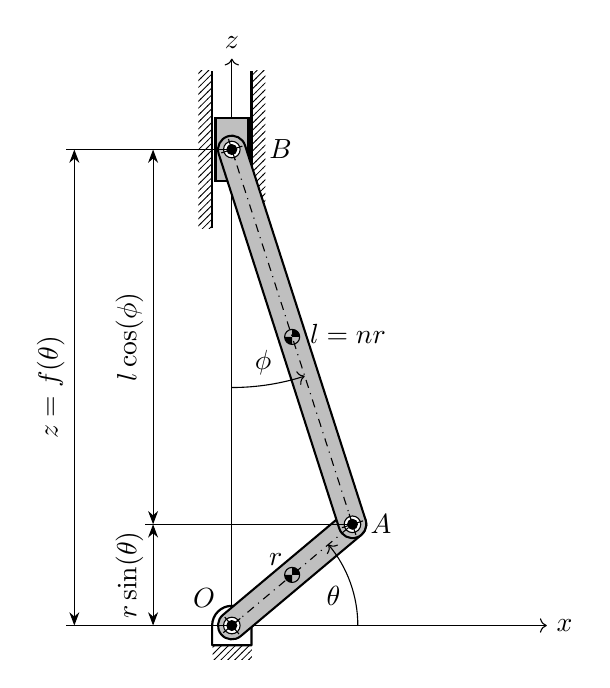
\begin{tikzpicture}
  % === Parameters ===
  \pgfmathsetmacro{\R}{2}           % Crank length r
  \pgfmathsetmacro{\N}{2.5}         % Link ratio n
  \pgfmathsetmacro{\Angle}{40}      % Crank angle in degrees
  % === Trig Evaluation ===
  \pgfmathsetmacro{\ct}{cos(\Angle)}
  \pgfmathsetmacro{\st}{sin(\Angle)}
  \pgfmathsetmacro{\asinfrac}{asin(\ct/\N)} % arcsin(cos(theta)/n)
  \pgfmathsetmacro{\cosarc}{cos(\asinfrac)} % cos(arcsin(...))
  \pgfmathsetmacro{\Yval}{\R*\st + \N*\R*\cosarc} % Final y pos of slider
  % === Coordinates ===
  \coordinate (O) at (0,0);
  % === Axes ===
  \draw[->] (O) -- ++({\R*2},0) node[right] {$x$};
  \draw[->] (O) -- ++(0,{\R*(\N+1.1)}) node[above] {$z$};
  % === Ground and Crank ===
  \pic (base) at (O) {frame pivot rounded};
  \pic (crank_arm) at (O) {link bar generic={\Angle:\R cm/1/1/1/1}};
  % === Slider and Connecting Rod ===
  \pic (slider) at (0,\Yval) [rotate=90] {frame dual pivot slide={2cm/0.0/0.4}};
  \pic (connecting_rod) at (crank_arm-end) {link bar generic={slider-center/1/1/1/1}};
  % === Labels and Geometry ===
  \draw[dashdotted] (O) -- (crank_arm-end) node[midway,above left] {$r$};
  \draw[dashdotted] (crank_arm-end) -- (slider-center) node[midway,above, right, xshift=3pt, yshift=1pt] {$l=nr$};
  \fill (O) circle (2pt)node[ xshift=-10pt, yshift=10pt] {$O$};
  \fill (crank_arm-end) circle (2pt)
    node[ right=3pt]{$A$};
    % {$(r\cos\theta,\ r\sin\theta)$};
  \fill (slider-center) circle (2pt)
    node[ right=10pt, align=left] {$B$};
      % {$(0,\ r\sin\theta +$\\$ \quad nr\cos\left(\arcsin\left(\frac{\cos\theta}{n}\right)\right))$};
  % Angle Arc
  \draw[->] ({\R*0.8},0) arc[start angle=0, end angle=\Angle, radius={\R*0.8}]
    node[midway,left,yshift=-5pt] {$\theta$};
  \draw[->] (0,{\Yval*0.5}) arc[start angle=-90, end angle=\asinfrac-90, radius={\Yval*0.5}]
    node[above,midway,xshift=-2pt] {$\phi$};
% Shared X for dimension and dash lines
\coordinate (dimX) at (-2.0, 0);
% solid horizontal lines at top and bottom
\draw[solid] ($(slider-center -| dimX) + (-0.1,0)$) -- (slider-center);
\draw[solid] ($(O -| dimX) + (-0.1,0)$) -- (O);
% One vertical dimension arrow from base to slider height
\draw[<->, >=Stealth] (dimX) -- (dimX |- slider-center)
  node[midway,sloped,rotate=0,above] {$z=f(\theta)$};
% Vertical arrow from (-1, 0) to (-1, r*sin(angle))
\draw[<->, >=Stealth] (-1, 0) -- (-1, {\R*\st})
    node[midway,sloped,above] {$r\sin(\theta)$};
% Vertical arrow from (-1, r*sin(angle)) to (-1, \Yval)
\draw[<->, >=Stealth] (-1, {\R*\st}) -- (-1, \Yval)
    node[midway,sloped,above] {$l\cos(\phi)$};
% Horizontal line from (-1, r*sin(angle)) to (r*cos(angle), r*sin(angle))
\draw[solid] (-1.1, {\R*\st}) -- ({\R*\ct}, {\R*\st})
    node[midway,below] {};
\end{tikzpicture}
    \caption{Slider-crank mechanism}
    \label{fig:SliderCrank}
\end{center}
\end{figure}

\subsubsection{Forward Kinematics:}

\noindent We consider a vertical slider--crank mechanism in which
a crank of length $r$drives a slider B via a connecting rod of length
$l$, The vertical displacement of the slider, $z$, can be written
as:

\noindent\begin{equation}
z = r \sin(\theta) + l\cos(\phi)
\end{equation}

\noindent Here, $\theta$ is the angle between the crank arm and the
horizontal $x$-axis, and $\phi$ is the angle between the connecting
rod and the vertical $z$-axis.

\noindent Applying the sine rule to $\triangle OAB$, we obtain :

\noindent\begin{equation}
\frac{r}{\sin(\phi)} = \frac{l}{\sin\left(\frac{\pi}{2} - \theta \right)}
\end{equation}

\noindent We define a ratio $n = l/r$ for convenience of calculation.
substituting $l=nr$ and solving for $\phi$ and we get-

\noindent\begin{equation}
\phi = \sin^{-1}\left( \frac{\cos\theta}{n} \right)
\end{equation}

\noindent So the displacement equation becomes -

\noindent\begin{equation}
  z = f(\theta)
  = r \sin(\theta) + nr\cos(\sin^{-1}\!(\frac{\cos\theta}{n}))
  \label{FK}
\end{equation}

\noindent Equation$\eqref{FK}$ gives the forward kinematics , the
vertical position $z$ of the slider as a function of crank angle
$\theta$.

\subsubsection{Inverse Kinematics:}

\noindent The inverse kinematics problem involves determining the
crank angle $\theta$ required to achieve a given vertical slider
position $z$. In $\triangle OAB$ applying cosine rule, we obtain
:

\noindent\begin{equation}
\angle AOB = \frac{\pi}{2} - \theta = \cos^{-1}\!(\frac{h^2 + r^2 - l^2}{2hr})
\end{equation}

\noindent substituting $l=nr$ and solving for $\theta$ and we obtain
-

\noindent\begin{equation}
\theta = \sin^{-1}\left( \frac{h^2 + r^2 (1- n^2)}{2hr} \right)
\label{eq:IK}
\end{equation}

\noindent This expression allows us to compute the crank angle $\theta$
given the slider displacement $h$.

\subsubsection{Inverse Dynamics:}

\noindent The dynamics of the system are derived using Lagrangian
mechanics. We consider the slider has a mass $m$ and the inertia
of motor driving the crank is $J$ in the crank frame. At this stage
of the analysis we assume the crank arm and the connecting rod has
no mass. In the $theta$ as the generalized co-ordinate system.

\noindent The total kinetic energy of the system can be written as:

\noindent\medskip{}

\noindent\begin{equation}
\begin{split}
    T &= T_{\rm motor} + T_{\rm slider} \\
      &= \tfrac{1}{2} J\,\dot{\theta}^2 + \tfrac{1}{2} m\,\dot{z}^2 \\
      &= \tfrac{1}{2} J\,\dot{\theta}^2 + \tfrac{1}{2} m\,\bigl( \tfrac{dz}{d\theta} \bigr)^2 \dot{\theta}^2 \\
      &= \tfrac{1}{2} \bigl( J + m\,\bigl( \tfrac{dz}{d\theta} \bigr)^2 \bigr) \dot{\theta}^2
\end{split}
\end{equation}

\noindent The potential energy of the system :

\noindent\medskip{}

\noindent\begin{equation}
  V = mgz = mgr(\sin(\theta) + n\cos(\sin^{-1}\!(\frac{\cos\theta}{n}))
\end{equation}

\noindent Hence the Lagrangian of the system is :

\noindent\medskip{}

\noindent\begin{equation}
\mathcal{L} = \tfrac{1}{2} \left( J + m \left( \tfrac{dz}{d\theta} \right)^2 \right) \dot{\theta}^2 - m g z(\theta)
\label{eq:L}
\end{equation}

\noindent For the generalized co-ordinate system $q$, the Euler-Lagrange
equations are:

\noindent\medskip{}

\noindent\begin{equation}
\frac{d}{dt} \left( \frac{\partial \mathcal{L}}{\partial \dot{\theta}} \right) - \frac{\partial \mathcal{L}}{\partial \theta} = Q
\end{equation}

\noindent Where, $Q$ represents the generalized force. For our system,
$q=\theta$, and thus required torque becomes $Q=\tau$ .Substituting
we get:

\noindent\medskip{}

\noindent\begin{equation}
\begin{aligned}
\tau 
&= \frac{d}{dt}\Bigl(\frac{\partial \mathcal{L}}{\partial \dot{\theta}}\Bigr)
  - \frac{\partial \mathcal{L}}{\partial \theta} \\[8pt]
&= \frac{d}{dt}\Bigl[(J + m\,(\frac{dz}{d\theta})^2)\,\dot{\theta}\Bigr]
  - \Bigl[\tfrac12\bigl(2m\,\frac{dz}{d\theta}\,\frac{d^2z}{d\theta^2}\bigr)\,\dot{\theta}^2
           - m g\,\frac{dz}{d\theta}\Bigr] \\[8pt]
&= (J + m\,(\frac{dz}{d\theta})^2)\,\ddot{\theta}
  + 2m\,\frac{dz}{d\theta}\,\frac{d^2z}{d\theta^2}\,\dot{\theta}^2
  - \bigl(m\,\frac{dz}{d\theta}\,\frac{d^2z}{d\theta^2}\,\dot{\theta}^2 
         - m g\,\frac{dz}{d\theta}\bigr) \\[6pt]
&= (J + m\,(\frac{dz}{d\theta})^2)\,\ddot{\theta}
  + m\,\frac{dz}{d\theta}\,\frac{d^2z}{d\theta^2}\,\dot{\theta}^2
  + m g\,\frac{dz}{d\theta}\,.
\end{aligned}
\label{eq:ID}
\end{equation}Here,

\noindent\begin{equation}
\begin{aligned}
\frac{dz}{d\theta}
  &= r\cos\theta
    + n r \biggl[-\sin\!\bigl(\sin^{-1}(\tfrac{\cos\theta}{n})\bigr)\;
      \frac{d}{d\theta}\sin^{-1}\!\bigl(\tfrac{\cos\theta}{n}\bigr)\biggr] 
    = r\cos\theta
    + \frac{r\,\cos\theta\,\sin\theta}{\sqrt{n^2-\cos^2\theta}},\\
\frac{d^2z}{d\theta^2}
  &= -r\sin\theta
    + r\Bigl(\frac{\cos2\theta}{\sqrt{n^2-\cos^2\theta}}
      - \frac{\cos^2\theta\,\sin^2\theta}{(n^2-\cos^2\theta)^{3/2}}\Bigr).
\end{aligned}
\end{equation}

\subsubsection{Optimal Configuration:}

In order replicate the torso motion as accurately as possible, we
must satisfy the position workspace requirements as well reproduce
the g-forces experienced by a runner.To satisfy the kinematics worksapce

The maximum g-force is experienced, vertically, when the runner is
at the lowest point in the trajectory. To generate maximum acceleration,
at the lowest point in the trajectory, the configuration dependent
load inertia of the system must match the motor inertia in the load
frame. From Equation $\ref{eq:ID}$ we find the the total effective
inertia of the system:

\begin{equation}
J_{total}  = J + m\,(\frac{dz}{d\theta})^2 = J + m(r\cos\theta+ \frac{r\,\cos\theta\,\sin\theta}{\sqrt{n^2-\cos^2\theta}})^2
\end{equation}

Therefore, the condition for inertia matching is 

\begin{equation}
y
\end{equation}


\end{document}
